To construct the matrix $\Pi \in \rea^{m \times n}$ we randomly select $s$ entries on each column to be non-zero and we set them to be $+\frac{1}{\sqrt{s}}$ or $-\frac{1}{\sqrt{s}}$ with equal probabilities. To formalize this we can use two sets of random variables $\delta_{r,i}$ and $\sigma_{r, i}$, where 

$$
 \delta_{r, i} = 
\begin{cases} 
    1 & \Pi_{r, i} \neq 0 \\
    0 & o.w
\end{cases}
$$
and 
$$
P(\sigma_{r, i} = 1) = P(\sigma_{r, i} = -1) = \frac{1}{2}.
$$
Using this notation, we can write the entries in $\Pi$ as $\Pi_{r, i} = \frac{1}{\sqrt{s}} \delta_{r, i} \sigma_{r, i}$, and proceed with the proof. 

The next step is to quantify the subspace embedding distortion error, which we want to bound by $\calO({\epsilon})$. 


\begin{fact}
    The OSE matrix $\Pi$ successfully embeds a subspace $S$ with an orthonormal basis $U$ if and only if 
    \begin{equation}
        \norm{(\Pi U)^T (\Pi U) - U^TU} \leq \epsilon
    \end{equation}
\end{fact}
\begin{proofsketch}


The reader can note that the spectral norm of a symmetric matrix $A$ is its largest eigenvalue, which can be written as $$ \norm{A} = \max_{\norm{e} = 1} {e^T A e}.$$

Therefore, the spectral norm of the symmetric matrix $(\Pi U)^T (\Pi U) - U^TU$ would be 
$$\norm{(\Pi U)^T (\Pi U) - U^TU} = \max_{\norm{e} = 1}{
     e^T ((\Pi U)^T (\Pi U) - U^TU) e }= \max_{\norm{e} = 1}{\norm{\Pi e}^2 - \norm{e}^2}$$

where, $\norm{\Pi e}^2 - \norm{e}^2$ is the distortion error of the subspace embedding, which we want to bound by $\calO({\epsilon})$. \cite{nelson2013osnap} provide an alternative way to think about this problem. It suffices to write $S$ as $$S = \{x : \exists y \in \rea^{d}, x = Uy\}.$$
Then $\Pi$ is an OSE if and only if $\norm{\Pi x} = (1 \pm \epsilon)\norm{x}$ with high probability. Note that $\norm{\Pi x} = \norm{\Pi U y}$, and since $U$ is a unitary matrix it preserves the norm, thus we have $$\norm{\Pi U y} = \norm{\Pi y} = (1 \pm \epsilon) \norm{y}.$$ 
This property is equivalent to having all the singular values of $\Pi U$ in the range of $(1 - \epsilon, 1 + \epsilon)$, meaning that the eigenvalues of $(\Pi U) ^ T (\Pi U)$ would be in the range of  $( (1 - \epsilon) ^ 2, (1 + \epsilon) ^ 2)$. Now since $U^T U = I$, then 
    $$(\Pi U) ^T (\Pi U) = I + ((\Pi U) ^T (\Pi U) - U^T U).$$
Following Weyl's inequality~\cite{nelson2013osnap} we can show that the eigenvalues of $(\Pi U) ^ T (\Pi U)$ are $1 \pm  \norm{(\Pi U)^T (\Pi U) - U^TU}$, which we need them to be in the range of $(-2\epsilon + \epsilon^2 + 1, 2\epsilon + \epsilon ^2 + 1)$. Consequently if $\epsilon$ is small enough, then $\norm{((\Pi U) ^T (\Pi U) - U^T U)} \leq 3 \epsilon = \calO{(\epsilon)}$

\end{proofsketch}

Now, we can continue the proof by reducing the spectral norm  $\norm{(\Pi U)^T (\Pi U) - U^TU}$ and find an upper bond on $m$ and $s$. One possible approach is to decompose $(\Pi U)^T (\Pi U)$ to its rows and use Matrix Chernoff concentration bound.

\begin{theorem}[MATRIX CHERNOFF]
    Let $A_i$ be independent random positive semi-definite matrices satisfying $\av[\sum{A_i}]= I$ and $\norm{A_i} \leq O(\frac{log(d / \delta)}{\epsilon ^ 2})$, then for any $\epsilon < 1$
   $$P(\norm{\sum A_i - I} \leq \epsilon) \geq 1 - \delta.$$
\end{theorem}
   To use the Matrix Chernoff bound, one can write the matrix $(\Pi U) ^ T (\Pi U)$ as the sum of random matrices:
\begin{equation}
    (\Pi U) ^ T (\Pi U) = \sum_{r}(\Pi U)_r (\Pi U)_r^{T}
\end{equation}
However, the norms of these uniform random matrices ($\norm{(\Pi U)_r ^ T (\Pi U)_r} = \norm{(\Pi U)_r}^{2}$) are not bounded, and they are also not independent. To handle this problem, we can  show that  the contribution of the off-diagonal terms in $(\Pi U)^T (\Pi U)$ gives us a set of new random matrices that are equivalent to the OSE error matrix $(\Pi U)^T (\Pi U) - U^TU$:

\begin{align*}
     (\Pi U) ^ T (\Pi U) & = \sum_{r}(\Pi U)_r {(\Pi U)_r}^{T} \\
     & = \frac{1}{s} \sum_{r} (\sum_{i} \delta_{r, i} \sigma_{r, i} u_i) (\sum_{i} \delta_{r, i} \sigma_{r, i} {u_i}^T) \\
     & = \frac{1}{s} \sum_{r} (\sum_{i} \delta_{r, i} u_i u_i ^T ) + (\sum_{i \neq j} \delta_{r, i} \delta_{r, j} \sigma_{r, i} \sigma_{r, j} u_i {u_j}^T) \\
     & \frac{1}{s} (\sum_{i} (\sum_{r} \delta_{r, i}) u_i {u_i}^T) + \frac{1}{s} (\sum_{r} (\sum_{i \neq j} \delta_{r, i} \delta_{r, j} \sigm_{r, i} \sigma_{r, j} u_i {u_j}^T) 
     \\
     & =  U^T U + \frac{1}{s} \sum_r \sum_{i \neq j} \delta_{r, i} \delta_{r, j} \sigma_{r,i} \sigma_{r, j} u_i {u_j}^{T}
\end{align*}

To find a bound on the spectral norm of $(\Pi U)^T (\Pi U) - U^TU$ we only need to find a matrix concentration bound on the contribution of rows in the off-diagonal entries. For each row, we now have to consider the collision incidents only, i.e., when multiple non-zero entries exist in a row of $\Pi$. We refer to these matrices by $Z_r$:
\begin{equation}
    (\Pi U)^T (\Pi U) - U^TU = \frac{1}{s} \sum_r \sum_{i \neq j} \delta_{r, i} \delta_{r, j} \sigma_{r,i} \sigma_{r, j} u_i u_j ^ T = \frac{1}{s} \sum_r {Z_r}.
\end{equation}
Even though the $Z_r$ variables are still not independent, we can use an alternative form of Matrix Chernoff bound with a
requirements on the conditional distribution of each random variable given the previous ones.
\begin{lemma}
\label{lemma_2}
    Let $A = \sum_i A_i$ be a sum of $m$ random symmetric matrices such that for all $i$ and all allowable values $A_1^{'}, A_2^{'}, \dots A_{i - 1}^{'}$,
    $$
        \norm{\av [cA_i | A_1^{'}, A_2^{'}, \dots A_{i - 1}^{'}]} \leq C  
    $$
then, 
$$
\av[\tr{\exp(cA)}] \leq d C^m.
$$
\end{lemma}

\begin{proof}

Define $S_{i}$ as the partial sum of $A_j$ matrices: $S_{i} = \sum_{j = 1}^{i}A_j$. Without loss of generality we can assume $c = 1$, since $cA_i = B_i$, where $B_i$'s are our new random symmetric matrices. Now, for $i > 0$

\begin{align*}
    \av[\tr{\exp(S_i)}] = &\av_{S_{i-1}}[\av_{A_i}[\tr{\exp(A_i + S_{i-1})}]] \\
    \leq & \av_{S_{i-1}}[\av_{A_i}[\tr{\exp(A_i}\exp(S_{i-1}))]] \\
    = & \av_{S_{i-1}}[\tr{\av_{A_i}[\exp(A_i)]\exp(S_{i-1})}] \\
    \leq & \av_{S_{i-1}}[\norm{\av_{A_i}[\exp(A_i)} \tr{\exp(S_{i-1})}] \\
    \leq & C\av[\tr{\exp(S_{i - 1})}]
\end{align*}
The second line is a result of the \textsc{Golden-Thompson} lemma that shows $$\tr{\exp(A + B)} \leq \tr{\exp(A)\exp(B)}.$$ 
The third line follows the linearity of trace and matrix product as $$\av_{S_{i - 1}}[\av_{A_i}[\tr{\exp(S_{i - 1})}]] = \av_{S_{i - 1}}[\tr{\exp(S_{i - 1})}].$$ 
We use the fact that for two positive semi-definite matrices $A$ and $B$, $\tr{A B} \leq \tr{A} \norm{B}$ to get the forth line, and by using lemma~\ref{exp_lemma}, we show that both $\exp(S_{i - 1})$ and $\av_{A_{i}}[\exp(A_i)]$ are positive semi-definite. Since by definition $\exp(0) = I$, then $\av[\tr{\exp(S_0)}] = d$, and, thus $\av[\tr{\exp(A)}] = dC^m$.
\end{proof}


\begin{lemma}
    The exponential of a symmetric matrix $A$ is positive semi-definite.
\label{exp_lemma}
\end{lemma}
\begin{proof}(Of lemma~\ref{exp_lemma})
    We have to show that $\exp(A)$ is positive semi-definite.
        Since $A$ is symmetric it is diagonalizable, and can write it as
        \begin{align*}
            &A  = P D P ^{-1}\\
            &\exp(A) = \sum_{k = 0}^{\infty} \frac{1}{K!} A^k\\
            &\exp(A) = \sum_{k = 0}^{\infty}  \frac{1}{K!} P D^k P^{-1} = P \exp(D) P^{-1}
        \end{align*}
    Now the eigenvalues of $\exp(A)$ are the values in the diagonal matrix $\exp(D)$ which are all positive. 
\end{proof}


Because the conditional norms of the $Z_r$'s are not bounded, we cannot use Lemma~\ref{lemma_2} directly.
For example, when each column of $\Pi$ has exactly $s - 1$ non-zero entries before the last row, then with the conditional probability of $1$, the last row of every column in $\Pi$ is non-zero, which makes the norm of the last $Z_r$ much larger than any constant value of $C$. This is because we would have to consider the contribution of \textbf{all} $u_i$ and $u_j$'s for any subspace:
\begin{align*}
    Z_r & = \sum_{i \neq j} \delta_{r,i} \delta_{r, j} \sigma_{r, i} \sigma_{r, j} u_i u_j ^T \\
    & =  \sum_{i \neq j} \sigma_{r, i} \sigma_{r, j} u_i u_j ^T
\end{align*}
This problem becomes particularly noticeable when conditioning on a large number of rows.
However, if we look at the first half of rows in $\Pi$, the conditional probability of each entry being non-zero does not surpass $\frac{s}{m/2}$, even if all the previous rows in the half matrix are non-zero, so we can simply split the $\sum_r Z_r$ to two halves. 

\begin{figure}
    \centering
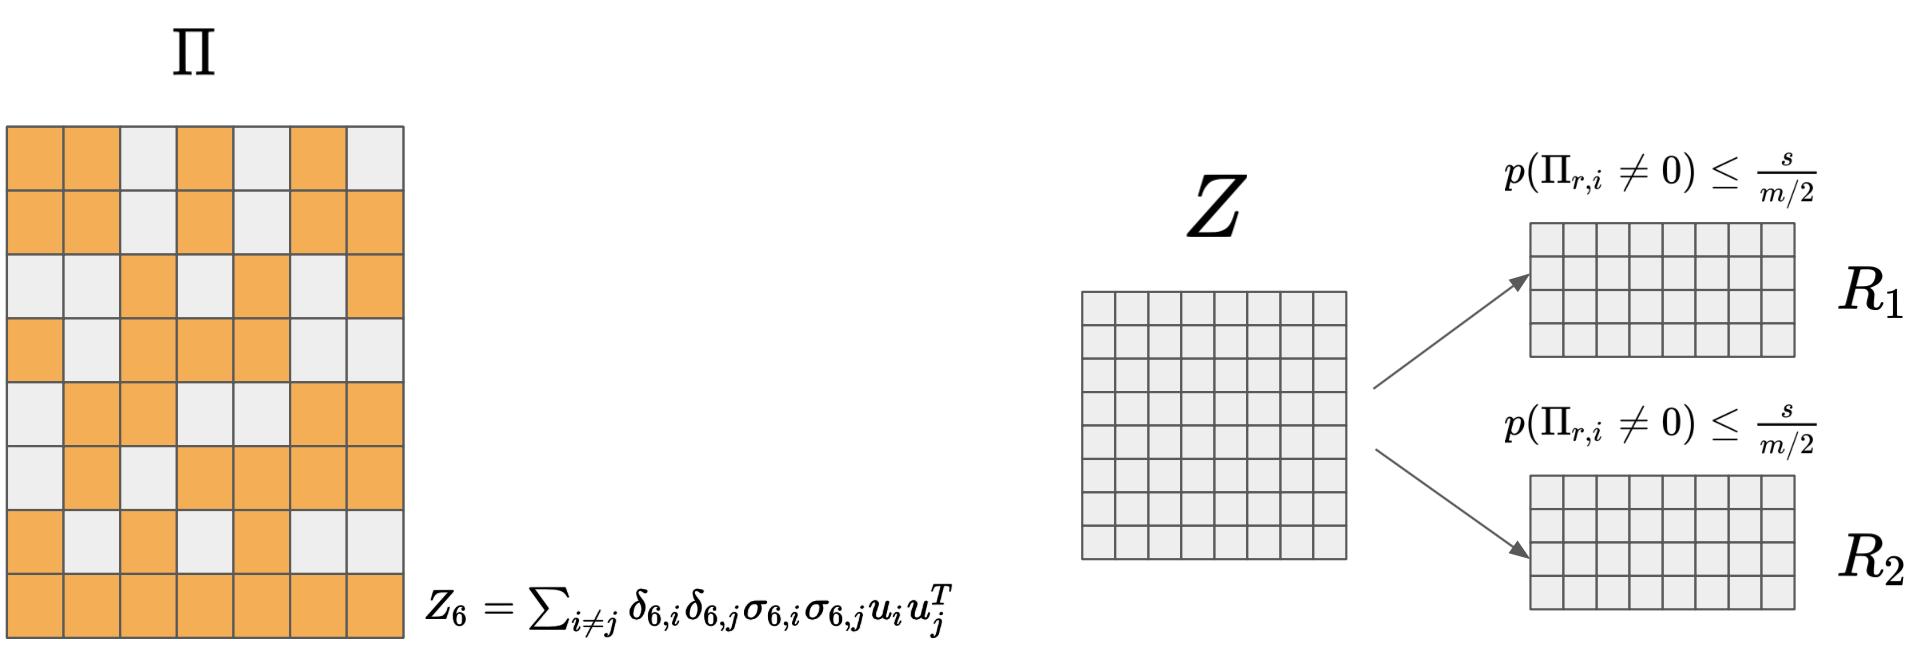
\includegraphics[width=15cm]{figures/splitting.png}
    \caption{Visualization of splitting the matrix to two halves. The orange boxes in matrix $\Pi$ specify the non-zero entries. Here $m = 8$ and $s = 5$. Each column of $\Pi$ has exactly $4$ non-zero entries before the last row.}
    \label{fig:splitting}
\end{figure}

\begin{equation}
    \sum_r Z_r = \sum_{r = 1}^{\frac{m}{2}} Z_r + \sum_{r = \frac{m}{2} + 1}^{m} Z_r = R_1 + R_2
\end{equation}
Even though $R_1$ and $R_2$ are not independent, we can apply Lemma~\ref{lemma_2} to each. The rest of the proof is straightforward. Using the \textsc{Golden-Thompson} lemma and the convexity of the trace, we can find an upper bound for $\av[\tr{\exp(c((\Pi U)^T (\Pi U) - U^TU))}]$ by decomposing it as the contribution of the two halves:
\begin{align*}
    \av[\tr{\exp(c((\Pi U)^T (\Pi U) - U^TU))}]  & \\ 
    &=  \av[\tr{\exp(\frac{c}{s}\sum_{r} Z_r)}] \\
    &= \av[\tr{\exp(\frac{c}{s}(R_1 + R_2))}]  \\ 
    & \leq \av[\tr{\exp(\frac{2c}{s}R_1)}]
\end{align*}
We can show that expected exponential value of the $Z_r$'s in the first half are bounded:
$$
    \av [\exp(\frac{2c}{s} Z_r)] \preceq (2 C^2 d + 1) I
$$
where $\norm{\exp(\frac{4c}{s} x_r {x_r}^{T}) - I } \leq C$ and $x_r = \sum_{i | w_i = 0} \delta_{r, i} \sigma_{r, i} u_i$ and $w_i$'s are $\B$-valued random variables with $P(w_i = 0) = P(w_i = 1) = \frac{1}{2}$. The complete proof for acquiring this bound can be found at~\cite[p6]{cohen2016nearly}.

Now that we have a bound on the expected values of $\exp(\frac{2c}{s} Z_r)$, we can apply Lemma~\ref{lemma_2} on all $Z_r$ variables in $R_1$ where $r \in 1, \dots, \frac{m}{2}$:
\begin{align*}
    \av[\norm{\exp(\frac{2c}{s} Z_r)}] \leq & 2C^2d + 1 \\ \leq & \exp(2C^2 d) \\ 
    \av[\tr{\exp(\frac{2c}{s} R_1)}] \leq & d \exp(C^2dm).
\end{align*}

Therefore,
$$
\av[\tr{\exp(c((\Pi U)^T (\Pi U) - U^TU))}] \leq d \exp(C^2dm).
$$

The following Theorem uses this bound to find the required number of rows $m$ and sparsity $s$ for $\Pi$ to be a subspace embedding. 


\begin{theorem}
    For any $B > 2$, $\delta < \frac{1}{2}$, $\epsilon < \frac{1}{2}$, a sparse embeddings matrix $\Pi$ with $m = O(\frac{Bd\log(d/\delta)}{\epsilon^2})$ and $s = O(\frac{\log_B(d/\delta)}{\epsilon})$ satisfies 
    \begin{equation}
        P(\norm{(\Pi U) ^ T (\Pi U) - U^T U} \leq \epsilon) \geq 1 - \delta
    \end{equation}
\label{main_theorem}
\end{theorem}
\begin{proofsketch}
    It suffices to fix a $c \propto \epsilon^{-1}\log(\frac{d}{\delta})$, such that $s/m \propto \epsilon / Bd$ and $c/s \propto \log B$ and $C^2 d m = 1$. Applying the above lemma to these $c$ and $C$ gives us 
    $$
    \av[\tr{\exp(\epsilon^{-1}\log(d/\delta)((\Pi U)^T (\Pi U) - U^TU) )}] \leq e d.
    $$

Now, we can write
\begin{align*}
        P(\norm{(\Pi U)^T \Pi U - U^TU} \geq \epsilon) & = P(\epsilon^{-1}\log(\frac{d}{\delta}) \norm{(\Pi U)^T \Pi U - U^TU} \geq \log(\frac{d}{\delta})) \\
        & = P(\exp(\epsilon^{-1}\log(\frac{d}{\delta}) \norm{(\Pi U)^T \Pi U - U^TU}) \geq \frac{d}{\delta}) \\
        & = P(\tr{\exp(\epsilon^{-1}\log(\frac{d}{\delta}) ((\Pi U)^T \Pi U - U^TU))} \geq \frac{d}{\delta}) \\
        & \leq \frac{\av[\tr{\exp(\epsilon^{-1}\log(d/\delta)((\Pi U)^T (\Pi U) - U^TU) )}]}{\frac{d}{\delta}} \\
        & \leq \frac{ed}{\frac{d}{\delta}} \\
        & = \calO({\delta})
        \\
          P(\norm{(\Pi U) ^ T (\Pi U) - U^T U} \leq \epsilon) & \geq 1 -  \calO({\delta})
\end{align*}
We can go from the second line to the third line by using lemma~\ref{exp_lemma}, which allows us to bound the spectral norm of the positive semi-definite matrix with its trace. Applying Markov's inequality on line 4 then gives us the desired bound.
 

\end{proofsketch}



